As described in \cref{sec-hw-early-evolution}, the GPU hardware architecture has undergone a drastic development, and still is.
This section presents the GPU hardware architecture as a conceptual GPGPU architecture.
The architecture is presented from a GPU computing point of view, meaning that some elements which are only used by the GPU for graphical purposes are not included.

The GPU hardware architecture consists of three main block categories:
\begin{itemize}
	\item Streaming Multiprocessors (SMs)
	\item Streaming Processors (SPs) 
	\item Memory (Local, Shared \& Global)
\end{itemize}

On a high level, the GPU can be described as an array of \textit{N} SMs, each consisting of \textit{M} cores (SPs) as illustrated on \cref{fig:hw-gpu}. 
The number of SMs contained in GPUs varies a lot, from small GPUs only containing a single SM, to the newest Nvidia architecture \textit{Tesla V100} containing 84 SMs \cite{Nvidia2017}.
The number of SMs, and thereby the number of SPs, contained in the GPU enables more tasks to be processed at the same time or a single task to be processed faster if enough parallelism is implemented for this given task.
Therefore, the future evolution of GPUs is focused on increasing the number of SMs and SPs.

In addition to the three main block categories presented above, three other blocks is also presented on \cref{fig:hw-gpu}, namely the \textit{Host Interface}, the \textit{Global Scheduler} and the \textit{Interconnection Network}.

%Host Interface
\textbf{The Host Interface} is the logical representation of the GPUs PCI Express port.
It implements functionality needed to perform CPU/GPU interactions. 
The Host Interface does so, by reading commands such as \textit{copying memory} and  \textit{launching Kernels} (further described in \cref{sec-pm-kernels}), and dispatches these commands to the appropriate hardware units.
In addition to command handling, the Host Interface also facilitates synchronization between the CPU and GPU. 
For more information regarding the Host Interface, and the interactions between the CPU see \cite{Wilt2013} chapter 2.5 - CPU/GPU Interactions.

%Global Scheduler
\textbf{The Global Scheduler}, also known as "GigaThread Engine" by Nvidia \cite{Nvidia2009}, is responsible of distributing threads to SMs, where they are executed.
Scheduling is done by splitting threads into thread blocks, which are further described in \cref{sec-pm-kernels}.
After the threads are split into blocks, they are assigned to the SMs by the Global Scheduler.
The Global Scheduler has to take several hardware constraints into consideration.
First a single block cannot be split between two SMs.
Also, each SM is limited in the amount of threads and blocks that can be scheduled to it. 
More information regarding how threads and blocks are optimized split between SMs is covered in \cref{ch-opti-intro}.

%Interconnection Network
\textbf{The Interconnection Network}, also known as "NoC", is a crossbar network.
It serves as communication channel both among the different SMs and between the individual SMs and the L2 Cache.




\begin{figure}[ht]
	\centering
	\fbox{
		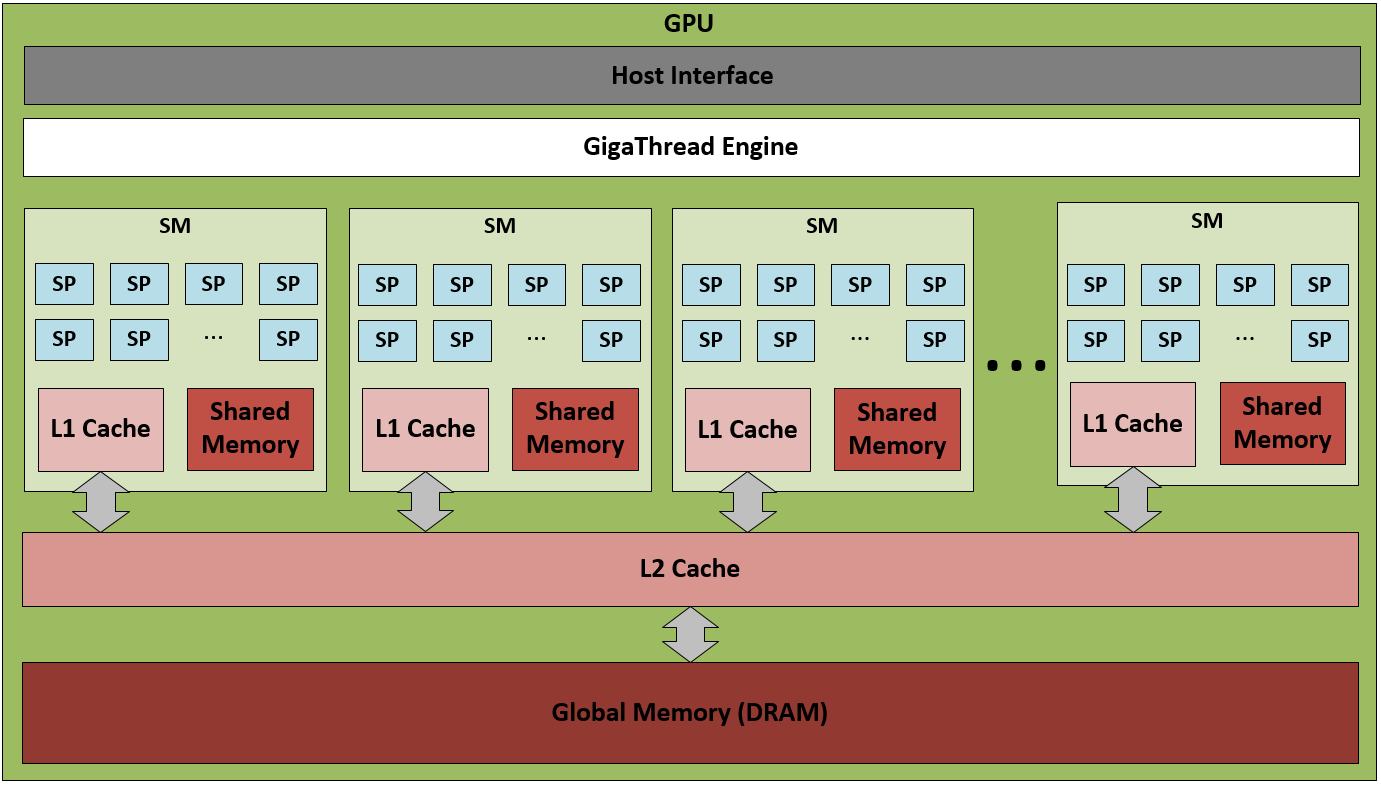
\includegraphics[width=1\textwidth]{figs/hw/hw-gpu}}
	\caption{Conceptual GPGPU hardware architecture}
	\label{fig:hw-gpu}
\end{figure}

Further information regarding SMs and SPs is covered in \cref{sec-hw-streaming-multiprocessors} and \cref{sec-hw-streaming-processors}.
Additional topics of the GPU hardware architecture is covered in the remaining subsections, including the memory model which is covered in \cref{sec-hw-memory-model}.